\documentclass[sigconf, screen, review, anonymous]{acmart}

\AtBeginDocument{%
  \providecommand\BibTeX{{%
    Bib\TeX}}}

\setcopyright{acmlicensed}
\copyrightyear{2026}
\acmYear{2026}
\acmDOI{XXXXXXX.XXXXXXX}

%%
%% ACM MM 2026
%%

%%
%% For managing citations, it is recommended to use bibliography
%% files in BibTeX format.
%%
\usepackage{natbib}

\usepackage{algorithm}
\usepackage{algorithmic}
\usepackage{pifont}
\usepackage{enumitem}
\usepackage{tabularx}
\usepackage{multirow}
\usepackage[normalem]{ulem}
\usepackage{booktabs}
\usepackage{amsmath}
\usepackage{amssymb}
\usepackage{bm}
\usepackage{colortbl}
\usepackage{color}
\usepackage{tabularray}
\usepackage{xspace}
\usepackage{makecell}

\begin{document}

%%
%% Title
%%
\title{StructRouter: Structure-Aware Multi-Agent Framework for Mixed-Mode Time Series Analysis}

\def\model{StructRouter\xspace}

% Math and result formatting
\newcommand{\update}[1]{{\textcolor{black}{#1}}}
\newcommand{\boldres}[1]{{\textbf{\textcolor{red}{#1}}}}
\newcommand{\secondres}[1]{{\underline{\textcolor{blue}{#1}}}}

% Algorithm macros
\newcommand{\Function}[2]{\STATE\textbf{function} \text{#1}$(#2)$}
\newcommand{\EndFunction}{\STATE\textbf{end function}}
\newcommand{\Comment}[1]{\STATE{\(\triangleright\) #1}}

%%
%% Anonymous authors for review
%%
\author{Anonymous Authors}

\settopmatter{printacmref=false}

%%
%% Abstract and main content
%%
\begin{abstract}
Time series forecasting is challenging when data exhibit mixed structural patterns that vary across segments. Existing mixture-of-experts (MoE) and Transformer approaches use hard routing that activates only expert subsets, leading to expert collapse and information loss. We propose \textbf{StructRouter}, which models time series as a mixture of learnable structural patterns with soft routing and interpretable causal communication. Our weight estimator combines MLP-based routing with prototype similarity: $w = \text{Softmax}(\text{MLP}(z) + \text{softplus}(\lambda) \cdot \text{Sim}(z, P))$, where $P \in \mathbb{R}^{K \times H}$ are orthogonal prototypes. All five experts contribute via $\text{Output} = \sum_i w_i \cdot \text{Expert}_i(x)$. Expert communication follows a Structural Causal Model with DAG constraint $h(W) = \text{tr}(\exp(W \odot W)) - N = 0$. A verification agent performs three-dimensional checks (consistency, validity, uncertainty) with gradient-aware rerouting when verification fails. We employ three-stage training (self-supervised $\rightarrow$ end-to-end $\rightarrow$ reinforcement fine-tuning) and RevIN for distribution shift handling. Evaluated on ETTh1/h2, ETTm1/m2, Weather, ECL, and Traffic, StructRouter achieves [TODO: fill after experiments]. Ablations demonstrate the contribution of each component.
\end{abstract}

\keywords{Time series forecasting, mixture of experts, soft routing, structural causal model}

\maketitle
\section{Introduction}

Time series analysis underpins critical applications across multimedia and intelligent systems: sensor streams from wearable devices, video analytics for traffic and surveillance, and IoT data from smart buildings and industrial monitoring. When such data exhibit \emph{mixed structural patterns}---trends, seasonality, regime shifts, and noise that vary across segments---forecasting becomes particularly challenging. A single model trained on homogeneous assumptions often fails to capture the diversity of patterns present in real-world time series.

Traditional methods make strong structural assumptions. ARIMA and exponential smoothing assume a single trend or seasonal decomposition~\cite{box2015time}. Spectral methods target periodicity. These approaches excel when the data match their assumptions but struggle when multiple patterns coexist or shift over time. Deep learning methods, especially Transformer-based architectures~\cite{vaswani2017attention}, treat all patterns uniformly through attention mechanisms. While flexible, they lack explicit structural modeling and can be data-inefficient when patterns are sparse or localized.

Mixture-of-experts (MoE) approaches, including Switch Transformer~\cite{fedus2022switch} and ST-MoE, address heterogeneity by routing inputs to specialized experts. However, they rely on \emph{hard routing}: only a small subset of experts is activated per input. This design leads to expert collapse (few experts dominate), information loss (inactive experts contribute nothing), and limited interpretability. Moreover, no existing framework jointly addresses three key aspects: (i) structure-aware pattern detection, (ii) soft expert routing that preserves full information, and (iii) interpretable inter-expert communication.

To bridge this gap, we propose \model, a structure-aware multi-agent framework for mixed-mode time series analysis. StructRouter models time series as a mixture of learnable structural patterns with soft routing and causal communication among experts. Our key design choices are:

\textbf{Structure-aware routing.} A learnable encoder extracts structural features from the input. Weight estimation fuses MLP-based routing with prototype similarity: $w = \text{Softmax}(\text{MLP}(z) + \text{softplus}(\lambda) \cdot \text{Sim}(z, P))$, where $P \in \mathbb{R}^{K \times H}$ are orthogonal pattern prototypes. Similar structural patterns receive similar routing weights, providing an inductive bias absent in purely data-driven MoE.

\textbf{Soft expert fusion.} Unlike hard routing, all five experts contribute in every forward pass: $\text{Output} = \sum_i w_i \cdot \text{Expert}_i(x)$. This avoids expert collapse and preserves full information for mixed-mode segments where multiple patterns coexist.

\textbf{Causal communication.} Experts (agents) communicate via a Structural Causal Model (SCM) with a learnable adjacency matrix $W_{\text{comm}}$ constrained to a Directed Acyclic Graph via the NOTEARS formulation: $h(W) = \text{tr}(\exp(W \odot W)) - N = 0$. The resulting DAG yields interpretable causal structure---which expert influences which---and supports do-calculus and counterfactual reasoning.

\textbf{Closed-loop verification.} A verification agent performs three-dimensional checks: Consistency (input--output structure alignment), Validity (statistical and range checks), and Uncertainty (aleatoric and epistemic via Monte Carlo dropout). When verification fails, an Inverse Consistency Check computes a suggested weight adjustment and triggers gradient-aware rerouting. The output retains gradients so that the consistency loss backpropagates through the prediction path, enabling the model to correct routing decisions in a closed loop.

\textbf{Progressive training.} We employ three-stage training: self-supervised structure learning, end-to-end supervised forecasting, and reinforcement fine-tuning (RFT). RevIN~\cite{kim2022reversible} handles distribution shift across segments.

Our main contributions are:

\begin{itemize}[leftmargin=*]
    \item \textbf{Multi-pattern weight estimation with prototype similarity.} We propose a weight estimator that fuses MLP-based routing with prototype similarity and orthogonal pattern prototypes. Combined with soft-weighted expert fusion, all experts contribute in every forward pass, avoiding expert collapse and preserving full information for mixed-mode time series.

    \item \textbf{SCM causal communication with DAG constraint.} We model expert communication as a Structural Causal Model with a learnable adjacency matrix constrained to a DAG via the NOTEARS formulation. This yields interpretable causal structure over experts and supports do-calculus and counterfactual reasoning, with parsimony through sparse regularization.

    \item \textbf{Closed-loop verification with gradient-aware rerouting.} We introduce a verification agent that performs three-dimensional checks (Consistency, Validity, Uncertainty). When verification fails, an Inverse Consistency Check triggers gradient-aware rerouting, with gradients flowing through the prediction path so the model can correct routing decisions in a closed loop.

    \item \textbf{Comprehensive empirical evaluation.} We conduct extensive experiments on seven benchmark datasets---ETTh1, ETTh2, ETTm1, ETTm2, Weather, ECL, and Traffic---under standard forecasting protocols (prediction lengths 96, 192, 336, 720). We provide ablations on soft vs.\ hard routing, DAG constraint, verification, and three-stage training, demonstrating the contribution of each component. The learned pattern prototypes and causal graphs offer interpretable insights into model behavior across domains.
\end{itemize}

\section{Related Work}

\subsection{Time Series Forecasting}

Traditional forecasting methods rely on strong structural assumptions. ARIMA~\cite{box2015time} and exponential smoothing (ETS)~\cite{hyndman2008forecasting} assume a single trend or seasonal decomposition. Spectral methods~\cite{welch1967use} target periodicity through Fourier or wavelet analysis. These approaches excel when the data match their assumptions but struggle when multiple patterns coexist or shift over time---a common scenario in real-world mixed-mode time series.

Deep learning has significantly advanced time series forecasting. Recurrent architectures such as DeepAR~\cite{salinas2019deepar} model temporal dependencies via autoregressive likelihood. Temporal Convolutional Networks (TCNs)~\cite{bai2018empirical} use causal convolutions for efficient sequence modeling. Transformer-based models have achieved state-of-the-art performance: Informer~\cite{zhou2021informer} and Autoformer~\cite{wu2021autoformer} address long-sequence efficiency; FEDformer~\cite{zhou2022fedformer} leverages frequency-domain decomposition; PatchTST~\cite{nie2022time} applies patch-based tokenization; iTransformer~\cite{liu2023itransformer} inverts the attention mechanism to treat variates as tokens. Despite their flexibility, these methods treat all patterns uniformly through attention or convolution and lack explicit modeling of mixed structural patterns.

\textbf{Gap:} No prior work explicitly models mixed structural patterns (trend, seasonality, regime shifts, noise) with learnable prototypes that guide routing. Existing deep learning methods either assume homogeneity or rely on implicit pattern discovery without structural inductive bias.

\subsection{Mixture of Experts for Time Series}

Mixture-of-experts (MoE) architectures route inputs to specialized sub-networks to handle heterogeneity. The classic MoE formulation~\cite{shazeer2017outrageously} uses a gating network to compute expert weights. Switch Transformer~\cite{fedus2022switch} reduces computation by routing each token to a single expert (top-1 routing), achieving scalability in large language models.

In time series, TimesFM~\cite{ekambaram2023timesfm} and TimeMixer~\cite{wang2023timemixer} apply MoE-style designs for forecasting. TimesFM uses a foundation model with mixture components; TimeMixer employs multi-scale mixing for decomposition. However, these approaches typically use \emph{hard routing}: only a subset of experts is activated per input. Hard routing leads to information loss (inactive experts contribute nothing), expert collapse (few experts dominate the routing distribution), and limited interpretability. Moreover, experts operate in isolation without explicit communication.

\textbf{Gap:} Hard routing loses information and exacerbates expert collapse. No prior time series MoE framework enables causal communication between experts or models their interactions through a structural causal model.

\subsection{Causal Discovery and Communication}

Causal discovery aims to learn directed acyclic graphs (DAGs) from observational data. NOTEARS~\cite{zheng2018dags} formulates DAG learning as a continuous optimization problem: the constraint $h(W) = \text{tr}(\exp(W \odot W)) - N = 0$ ensures acyclicity, enabling gradient-based learning of the adjacency matrix. This formulation has been extended to nonlinear settings and applied in various domains.

Multi-agent systems have explored communication protocols for cooperative learning. CommNet~\cite{sukhbaatar2016learning} allows agents to share a continuous communication vector. TarMAC~\cite{das2019tarmac} introduces targeted communication with attention-based addressing. These works focus on reinforcement learning and do not incorporate causal structure or time series forecasting.

\textbf{Gap:} No prior work combines SCM-based causal communication (with DAG constraints) with time series expert routing. The integration of NOTEARS-style DAG learning for inter-expert communication in a forecasting framework remains unexplored.

\section{Methodology}

In this section, we present \model, a structure-aware multi-agent framework for mixed-mode time series analysis. We describe each component with full mathematical detail, from problem formulation through the joint loss and three-stage training.

\subsection{Problem Formulation}
\label{sec:problem}

Let $\mathbf{x} \in \mathbb{R}^{L \times D}$ denote a multivariate time series input with lookback length $L$ and $D$ variates. The goal is to predict future values $\hat{\mathbf{y}} \in \mathbb{R}^{P \times D}$ for forecasting horizon $P$ (prediction length). \model learns to decompose $\mathbf{x}$ into $K$ structural patterns and route to specialized experts. Formally, we learn a mapping $f_\theta: \mathbf{x} \mapsto \hat{\mathbf{y}}$ that:
\begin{enumerate}[leftmargin=*]
    \item Encodes structural features from $\mathbf{x}$;
    \item Estimates soft routing weights over $K$ pattern prototypes;
    \item Fuses outputs from $K$ experts via soft weighting;
    \item Enables causal communication among experts via a DAG-constrained adjacency;
    \item Verifies predictions and adjusts routing when consistency fails.
\end{enumerate}

\subsection{Structure Encoder}
\label{sec:encoder}

The structure encoder extracts global and sequential representations from $\mathbf{x}$. We apply RevIN~\cite{kim2022reversible} for reversible instance normalization before encoding. The encoder comprises:

\textbf{Causal Temporal Convolution.} We use CausalConv1d layers with exponential dilation $d_l = 2^l$ for layer $l$, ensuring no future leakage:
\begin{equation}
\mathbf{H}^{(0)} = \text{CausalConv1d}(\mathbf{x}), \quad \mathbf{H}^{(l)} = \sigma(\text{CausalConv1d}_l(\mathbf{H}^{(l-1)})).
\end{equation}

\textbf{Multi-Head Self-Attention.} The convolutional features are passed through multi-head self-attention~\cite{vaswani2017attention}:
\begin{equation}
\mathbf{H}_{\text{attn}} = \text{LayerNorm}(\mathbf{H}^{(L)} + \text{MultiHeadAttn}(\mathbf{H}^{(L)})).
\end{equation}

\textbf{Statistics Fusion.} We extract statistics features: mean $\boldsymbol{\mu}$, standard deviation $\boldsymbol{\sigma}$, trend (linear regression slope), change intensity (temporal variance of differences), and autocorrelation at lag 1. These are projected and fused:
\begin{equation}
\mathbf{z}_{\text{stats}} = \text{MLP}([\boldsymbol{\mu}; \boldsymbol{\sigma}; \text{trend}; \text{change\_intensity}; \text{autocorr}]).
\end{equation}

\textbf{Pooling and Output.} The final encoder outputs are:
\begin{align}
\mathbf{z}_{\text{global}} &= \frac{1}{2}\left( \text{avgpool}(\mathbf{H}_{\text{attn}}) + \text{maxpool}(\mathbf{H}_{\text{attn}}) \right) + \mathbf{z}_{\text{stats}} \in \mathbb{R}^H, \\
\mathbf{z}_{\text{seq}} &= \mathbf{H}_{\text{attn}} \in \mathbb{R}^{L \times H}.
\end{align}
where $H$ is the hidden dimension. We denote $\mathbf{z} = \mathbf{z}_{\text{global}}$ for routing.

\subsection{Multi-Pattern Weight Estimation (C1)}
\label{sec:weight}

The weight estimator fuses MLP-based routing with prototype similarity. Let $\mathbf{P} \in \mathbb{R}^{K \times H}$ denote $K$ orthogonal pattern prototypes, initialized via $\texttt{nn.init.orthogonal\_}$.

\textbf{Similarity.} We compute cosine similarity between the encoded representation and prototypes, with learned normalization:
\begin{equation}
\text{Sim}(\mathbf{z}, \mathbf{P}) = \mathbf{z}_{\text{norm}} \cdot \mathbf{P}_{\text{norm}}^\top \in \mathbb{R}^K,
\end{equation}
where $\mathbf{z}_{\text{norm}}$ and $\mathbf{P}_{\text{norm}}$ are L2-normalized (optionally with a learned linear transform).

\textbf{Core Formula.} The routing weights are:
\begin{equation}
\label{eq:weight}
\mathbf{w} = \text{Softmax}\left( \frac{\text{MLP}(\mathbf{z}) + \text{softplus}(\lambda) \cdot \text{Sim}(\mathbf{z}, \mathbf{P})}{\tau} \right),
\end{equation}
where $\lambda \in \mathbb{R}$ is a learnable balance parameter, $\tau$ is temperature, and $\mathbf{w} \in \mathbb{R}^K$ sums to 1.

\textbf{Prototype Orthogonality Regularization.} To encourage diversity among prototypes, we add:
\begin{equation}
\label{eq:ortho}
\mathcal{L}_{\text{ortho}} = \left\| \mathbf{P}_{\text{norm}}^\top \mathbf{P}_{\text{norm}} - \mathbf{I} \right\|_F^2.
\end{equation}

\subsection{Soft-Weighted Expert Fusion (C2)}
\label{sec:fusion}

Unlike hard routing, all experts contribute in every forward pass:
\begin{equation}
\label{eq:fusion}
\text{Output} = \sum_{i=1}^{K} w_i \cdot \text{Expert}_i(\mathbf{x}) + \text{Residual}(\mathbf{x}).
\end{equation}

We use five experts: \textbf{Periodic} (FFT-based frequency decomposition), \textbf{Trend} (linear decomposition), \textbf{Noise} (denoising autoencoder), \textbf{Abrupt} (change-point sensitive), and \textbf{General} (MLP). Expert dropout is applied for regularization during training.

\subsection{SCM Causal Communication (C4)}
\label{sec:causal}

Experts are treated as agents. We stack their outputs into agent states $\mathbf{S} \in \mathbb{R}^{B \times N \times H}$ where $N$ is the number of agents (experts). Message passing updates agent $j$ as:
\begin{equation}
\label{eq:message}
\mathbf{S}_j^{\text{new}} = \mathbf{S}_j^{\text{old}} + \text{gate} \cdot \text{Receive}\left( \sum_{i} W[i,j] \cdot \text{Message}(\mathbf{S}_i) \right).
\end{equation}

The communication matrix $\mathbf{W}_{\text{comm}} \in \mathbb{R}^{N \times N}$ is constrained as follows:
\begin{itemize}[leftmargin=*]
    \item \textbf{Softmax normalization} along the sender dimension so that $\sum_i W[i,j] = 1$ (or similar normalization);
    \item \textbf{Diagonal masking}: $W[j,j] = 0$ (no self-loops);
    \item \textbf{DAG constraint} via NOTEARS~\cite{zheng2018dags}:
    \begin{equation}
    \label{eq:dag}
    h(\mathbf{W}) = \text{tr}(\exp(\mathbf{W} \odot \mathbf{W})) - N = 0;
    \end{equation}
    \item \textbf{Clamping}: $\mathbf{W}$ is clamped to $[-2, 2]$ for numerical stability.
\end{itemize}

The matrix $\mathbf{W}$ is learned jointly with the rest of the model; $h(\mathbf{W}) = 0$ is enforced via a penalty term in the loss.

\subsection{Verification Agent (C6)}
\label{sec:verification}

The verification agent performs a three-dimensional check:

\textbf{1. Consistency.} We compute cosine similarity between input structure $\mathbf{S}_{\text{in}}$ and output structure $\mathbf{S}_{\text{out}}$, plus a learned consistency score:
\begin{equation}
c_{\text{consist}} = \cos(\mathbf{S}_{\text{in}}, \mathbf{S}_{\text{out}}) + \text{MLP}_{\text{score}}([\mathbf{S}_{\text{in}}; \mathbf{S}_{\text{out}}]).
\end{equation}

\textbf{2. Validity.} Statistical checks on the prediction: range (within expected bounds), outliers (z-score), skewness. A binary or scalar validity score $c_{\text{valid}}$ is produced.

\textbf{3. Uncertainty.} Monte Carlo dropout yields aleatoric and epistemic uncertainty estimates:
\begin{equation}
c_{\text{uncertainty}} = f(\sigma_{\text{aleatoric}}, \sigma_{\text{epistemic}}).
\end{equation}

\textbf{Inverse Consistency Check.} When verification fails, we compute suggested weights $\mathbf{w}_{\text{suggested}}$ via a learned adjustment module. Gradient-aware rerouting: compute $\hat{\mathbf{y}}_2$ with $\mathbf{w}_{\text{suggested}}$, then mix with the original prediction using detached confidence:
\begin{equation}
\hat{\mathbf{y}}_{\text{final}} = (1 - \alpha) \cdot \hat{\mathbf{y}}_1 + \alpha \cdot \hat{\mathbf{y}}_2, \quad \alpha = \text{detach}(\text{confidence}).
\end{equation}

\textbf{Gradient fix:} The output structure retains gradients (only the mixing coefficient $\alpha$ is detached). The input to the adjustment is detached so that gradients flow through the prediction path, enabling the model to correct routing in a closed loop.

\subsection{Joint Loss Function (C7)}
\label{sec:loss}

The total loss is:
\begin{equation}
\label{eq:total_loss}
\mathcal{L}_{\text{total}} = \mathcal{L}_{\text{task}} + \alpha \mathcal{L}_{\text{consist}} + \beta \mathcal{L}_{\text{sparse}} + \gamma(t) \mathcal{L}_{\text{causal}} + \delta \mathcal{L}_{\text{balance}} + \varepsilon \mathcal{L}_{\text{ortho}}.
\end{equation}

\textbf{Task loss.} $\mathcal{L}_{\text{task}} = \text{MSE}(\hat{\mathbf{y}}, \mathbf{y})$ or MAE for forecasting.

\textbf{Consistency loss.} $\mathcal{L}_{\text{consist}}$ penalizes low consistency scores from the verification agent.

\textbf{Sparse regularization.} $\mathcal{L}_{\text{sparse}} = \|\mathbf{W}_{\text{comm}}\|_1$ encourages sparse causal graphs.

\textbf{DAG penalty with warmup.} $\mathcal{L}_{\text{causal}} = h(\mathbf{W})^2$. The weight $\gamma(t)$ uses linear warmup:
\begin{equation}
\label{eq:gamma}
\gamma(t) = \gamma_{\text{target}} \cdot \min\left( \frac{\text{step}}{\text{warmup\_steps}}, 1 \right).
\end{equation}
This avoids DAG penalty explosion early in training.

\textbf{Expert balance loss.} To prevent expert collapse, we use variance of mean usage across the batch plus an auxiliary load-balancing loss (Switch Transformer style~\cite{fedus2022switch}):
\begin{equation}
\mathcal{L}_{\text{balance}} = \text{Var}(\bar{\mathbf{w}}_{\text{batch}}) + \mathcal{L}_{\text{aux}},
\end{equation}
where $\bar{\mathbf{w}}_{\text{batch}}$ is the mean routing weight per expert over the batch.

\textbf{Prototype orthogonality.} $\mathcal{L}_{\text{ortho}}$ is defined in Eq.~\eqref{eq:ortho} to encourage prototype diversity.

\subsection{Three-Stage Training (C8)}
\label{sec:training}

\textbf{Stage 1: Self-Supervised.} Train the encoder and weight estimator only. Objectives: contrastive loss (similar segments have similar $\mathbf{z}$), mask reconstruction (predict masked tokens), and structure prediction (predict statistics from $\mathbf{z}$). No expert or causal modules are trained.

\textbf{Stage 2: End-to-End.} Train the full model with $\mathcal{L}_{\text{total}}$. Use per-module learning rates: slower for weight estimator prototypes, faster for $\mathbf{W}_{\text{comm}}$. Apply gradient clipping. LR warmup (e.g., 10 epochs) followed by cosine annealing.

\textbf{Stage 3: Reinforcement Fine-Tuning (RFT).} Freeze the backbone (encoder, experts). Train the router (weight estimator) and tool adapter with PPO. The reward reflects forecasting accuracy and verification consistency.

\subsection{RevIN Integration}
\label{sec:revin}

We apply RevIN~\cite{kim2022reversible} for reversible instance normalization. Before the encoder:
\begin{equation}
\mathbf{x}_{\text{norm}} = \frac{\mathbf{x} - \boldsymbol{\mu}_{\text{inst}}}{\boldsymbol{\sigma}_{\text{inst}} + \epsilon},
\end{equation}
where $\boldsymbol{\mu}_{\text{inst}}$ and $\boldsymbol{\sigma}_{\text{inst}}$ are computed per instance (along the time dimension). After the prediction head:
\begin{equation}
\hat{\mathbf{y}} = \hat{\mathbf{y}}_{\text{raw}} \cdot \boldsymbol{\sigma}_{\text{inst}} + \boldsymbol{\mu}_{\text{inst}}.
\end{equation}
Learnable affine parameters can be added for channel-wise scaling. RevIN mitigates distribution shift across segments and improves convergence.

\section{Experiments}

We conduct comprehensive experiments to evaluate \model on seven benchmark datasets for long-term time series forecasting. We compare against eight state-of-the-art baselines, perform ablations to isolate the contribution of each component, and provide analysis of expert behavior, causal structure, and efficiency.

\subsection{Experimental Setup}

\paragraph{Datasets.}
We evaluate on seven widely-used benchmarks spanning diverse domains and variable counts. \textbf{ETTh1} and \textbf{ETTh2}~\cite{zhou2021informer} are hourly electricity transformer temperature data with 7 variables. \textbf{ETTm1} and \textbf{ETTm2} are 15-minute resolution variants with 7 variables. \textbf{Weather} contains 21 meteorological variables. \textbf{ECL} (Electricity)~\cite{wu2021autoformer} comprises 321 electricity load series. \textbf{Traffic}~\cite{wu2021autoformer} includes 862 traffic occupancy series. We follow standard chronological splits: 6:2:2 (train/val/test) for ETT datasets and 7:1:2 for Weather, ECL, and Traffic. Input length is 336 time steps (96 for ETTh1/ETTh2 due to shorter history). We evaluate prediction lengths $\{96, 192, 336, 720\}$.

\paragraph{Baselines.}
We compare against eight state-of-the-art forecasting methods: \textbf{iTransformer}~\cite{liu2024itransformer} with inverted variate-wise attention; \textbf{PatchTST}~\cite{nie2023patchtst} with patch-based tokenization; \textbf{TimesNet}~\cite{wu2023timesnet} with multi-scale 2D-variation modeling; \textbf{FEDformer}~\cite{zhou2022fedformer} with frequency-domain decomposition; \textbf{Autoformer}~\cite{wu2021autoformer} with auto-correlation; \textbf{DLinear}~\cite{zeng2023dlinear} with simple linear decomposition; \textbf{SCINet}~\cite{liu2022scinet} with sample convolution; and \textbf{Crossformer}~\cite{zhang2023crossformer} with cross-dimension attention.

\paragraph{Metrics.}
We report \textbf{MSE} (Mean Squared Error) and \textbf{MAE} (Mean Absolute Error), following standard practice in long-term forecasting benchmarks.

\paragraph{Implementation.}
\model is implemented in PyTorch with hidden dimension 256, 5 experts, and RevIN~\cite{kim2022reversible} enabled for distribution normalization. We employ three-stage training: (1) self-supervised structure learning on the encoder and weight estimator; (2) end-to-end supervised forecasting; (3) reinforcement fine-tuning (RFT)~\cite{schulman2017ppo} of the weight estimator with frozen experts. Batch size [TODO], epochs [TODO], learning rate [TODO], and optimizer [TODO] are specified in the appendix.

\subsection{Main Results}

Table~\ref{tab:main_results} presents long-term forecasting results across all datasets and prediction lengths. \model achieves competitive or state-of-the-art performance on most settings. On ETTh1 and ETTh2, the structure-aware routing and soft expert fusion effectively capture mixed patterns in electricity data. On high-variate datasets (ECL, Traffic), the prototype-based weight estimation and causal communication scale well to diverse variable structures. Results are averaged over 3 runs.

\begin{table*}[t]
\centering
\caption{Long-term forecasting results (MSE/MAE) across all datasets and prediction lengths. Best in \boldres{bold red}, second best in \secondres{underlined blue}. Results averaged over 3 runs.}
\label{tab:main_results}
\resizebox{\linewidth}{!}{
\begin{tabular}{l|cc|cc|cc|cc|cc|cc|cc|cc|cc|cc|cc|cc|cc|cc|cc|cc|cc|cc|cc|cc|cc|cc|cc|cc|cc|cc}
\toprule[1.5pt]
\multirow{3}{*}{Method} & \multicolumn{8}{c|}{ETTh1} & \multicolumn{8}{c|}{ETTh2} & \multicolumn{8}{c|}{ETTm1} & \multicolumn{8}{c|}{ETTm2} & \multicolumn{8}{c|}{Weather} & \multicolumn{8}{c|}{ECL} & \multicolumn{8}{c}{Traffic} \\
\cmidrule(lr){2-9} \cmidrule(lr){10-17} \cmidrule(lr){18-25} \cmidrule(lr){26-33} \cmidrule(lr){34-41} \cmidrule(lr){42-49} \cmidrule(lr){50-57}
 & \multicolumn{2}{c}{96} & \multicolumn{2}{c}{192} & \multicolumn{2}{c}{336} & \multicolumn{2}{c}{720} & \multicolumn{2}{c}{96} & \multicolumn{2}{c}{192} & \multicolumn{2}{c}{336} & \multicolumn{2}{c}{720} & \multicolumn{2}{c}{96} & \multicolumn{2}{c}{192} & \multicolumn{2}{c}{336} & \multicolumn{2}{c}{720} & \multicolumn{2}{c}{96} & \multicolumn{2}{c}{192} & \multicolumn{2}{c}{336} & \multicolumn{2}{c}{720} & \multicolumn{2}{c}{96} & \multicolumn{2}{c}{192} & \multicolumn{2}{c}{336} & \multicolumn{2}{c}{720} & \multicolumn{2}{c}{96} & \multicolumn{2}{c}{192} & \multicolumn{2}{c}{336} & \multicolumn{2}{c}{720} & \multicolumn{2}{c}{96} & \multicolumn{2}{c}{192} & \multicolumn{2}{c}{336} & \multicolumn{2}{c}{720} \\
 & MSE & MAE & MSE & MAE & MSE & MAE & MSE & MAE & MSE & MAE & MSE & MAE & MSE & MAE & MSE & MAE & MSE & MAE & MSE & MAE & MSE & MAE & MSE & MAE & MSE & MAE & MSE & MAE & MSE & MAE & MSE & MAE & MSE & MAE & MSE & MAE & MSE & MAE & MSE & MAE & MSE & MAE & MSE & MAE & MSE & MAE & MSE & MAE & MSE & MAE & MSE & MAE & MSE & MAE & MSE & MAE & MSE & MAE \\
\midrule
iTransformer~\cite{liu2024itransformer} & [TODO] & [TODO] & [TODO] & [TODO] & [TODO] & [TODO] & [TODO] & [TODO] & [TODO] & [TODO] & [TODO] & [TODO] & [TODO] & [TODO] & [TODO] & [TODO] & [TODO] & [TODO] & [TODO] & [TODO] & [TODO] & [TODO] & [TODO] & [TODO] & [TODO] & [TODO] & [TODO] & [TODO] & [TODO] & [TODO] & [TODO] & [TODO] & [TODO] & [TODO] & [TODO] & [TODO] & [TODO] & [TODO] & [TODO] & [TODO] & [TODO] & [TODO] & [TODO] & [TODO] & [TODO] & [TODO] & [TODO] & [TODO] & [TODO] & [TODO] & [TODO] & [TODO] & [TODO] & [TODO] & [TODO] & [TODO] & [TODO] & [TODO] \\
PatchTST~\cite{nie2023patchtst} & [TODO] & [TODO] & [TODO] & [TODO] & [TODO] & [TODO] & [TODO] & [TODO] & [TODO] & [TODO] & [TODO] & [TODO] & [TODO] & [TODO] & [TODO] & [TODO] & [TODO] & [TODO] & [TODO] & [TODO] & [TODO] & [TODO] & [TODO] & [TODO] & [TODO] & [TODO] & [TODO] & [TODO] & [TODO] & [TODO] & [TODO] & [TODO] & [TODO] & [TODO] & [TODO] & [TODO] & [TODO] & [TODO] & [TODO] & [TODO] & [TODO] & [TODO] & [TODO] & [TODO] & [TODO] & [TODO] & [TODO] & [TODO] & [TODO] & [TODO] & [TODO] & [TODO] & [TODO] & [TODO] & [TODO] & [TODO] & [TODO] & [TODO] \\
TimesNet~\cite{wu2023timesnet} & [TODO] & [TODO] & [TODO] & [TODO] & [TODO] & [TODO] & [TODO] & [TODO] & [TODO] & [TODO] & [TODO] & [TODO] & [TODO] & [TODO] & [TODO] & [TODO] & [TODO] & [TODO] & [TODO] & [TODO] & [TODO] & [TODO] & [TODO] & [TODO] & [TODO] & [TODO] & [TODO] & [TODO] & [TODO] & [TODO] & [TODO] & [TODO] & [TODO] & [TODO] & [TODO] & [TODO] & [TODO] & [TODO] & [TODO] & [TODO] & [TODO] & [TODO] & [TODO] & [TODO] & [TODO] & [TODO] & [TODO] & [TODO] & [TODO] & [TODO] & [TODO] & [TODO] & [TODO] & [TODO] & [TODO] & [TODO] & [TODO] & [TODO] \\
FEDformer~\cite{zhou2022fedformer} & [TODO] & [TODO] & [TODO] & [TODO] & [TODO] & [TODO] & [TODO] & [TODO] & [TODO] & [TODO] & [TODO] & [TODO] & [TODO] & [TODO] & [TODO] & [TODO] & [TODO] & [TODO] & [TODO] & [TODO] & [TODO] & [TODO] & [TODO] & [TODO] & [TODO] & [TODO] & [TODO] & [TODO] & [TODO] & [TODO] & [TODO] & [TODO] & [TODO] & [TODO] & [TODO] & [TODO] & [TODO] & [TODO] & [TODO] & [TODO] & [TODO] & [TODO] & [TODO] & [TODO] & [TODO] & [TODO] & [TODO] & [TODO] & [TODO] & [TODO] & [TODO] & [TODO] & [TODO] & [TODO] & [TODO] & [TODO] & [TODO] & [TODO] \\
Autoformer~\cite{wu2021autoformer} & [TODO] & [TODO] & [TODO] & [TODO] & [TODO] & [TODO] & [TODO] & [TODO] & [TODO] & [TODO] & [TODO] & [TODO] & [TODO] & [TODO] & [TODO] & [TODO] & [TODO] & [TODO] & [TODO] & [TODO] & [TODO] & [TODO] & [TODO] & [TODO] & [TODO] & [TODO] & [TODO] & [TODO] & [TODO] & [TODO] & [TODO] & [TODO] & [TODO] & [TODO] & [TODO] & [TODO] & [TODO] & [TODO] & [TODO] & [TODO] & [TODO] & [TODO] & [TODO] & [TODO] & [TODO] & [TODO] & [TODO] & [TODO] & [TODO] & [TODO] & [TODO] & [TODO] & [TODO] & [TODO] & [TODO] & [TODO] & [TODO] & [TODO] \\
DLinear~\cite{zeng2023dlinear} & [TODO] & [TODO] & [TODO] & [TODO] & [TODO] & [TODO] & [TODO] & [TODO] & [TODO] & [TODO] & [TODO] & [TODO] & [TODO] & [TODO] & [TODO] & [TODO] & [TODO] & [TODO] & [TODO] & [TODO] & [TODO] & [TODO] & [TODO] & [TODO] & [TODO] & [TODO] & [TODO] & [TODO] & [TODO] & [TODO] & [TODO] & [TODO] & [TODO] & [TODO] & [TODO] & [TODO] & [TODO] & [TODO] & [TODO] & [TODO] & [TODO] & [TODO] & [TODO] & [TODO] & [TODO] & [TODO] & [TODO] & [TODO] & [TODO] & [TODO] & [TODO] & [TODO] & [TODO] & [TODO] & [TODO] & [TODO] & [TODO] & [TODO] \\
SCINet~\cite{liu2022scinet} & [TODO] & [TODO] & [TODO] & [TODO] & [TODO] & [TODO] & [TODO] & [TODO] & [TODO] & [TODO] & [TODO] & [TODO] & [TODO] & [TODO] & [TODO] & [TODO] & [TODO] & [TODO] & [TODO] & [TODO] & [TODO] & [TODO] & [TODO] & [TODO] & [TODO] & [TODO] & [TODO] & [TODO] & [TODO] & [TODO] & [TODO] & [TODO] & [TODO] & [TODO] & [TODO] & [TODO] & [TODO] & [TODO] & [TODO] & [TODO] & [TODO] & [TODO] & [TODO] & [TODO] & [TODO] & [TODO] & [TODO] & [TODO] & [TODO] & [TODO] & [TODO] & [TODO] & [TODO] & [TODO] & [TODO] & [TODO] & [TODO] & [TODO] \\
Crossformer~\cite{zhang2023crossformer} & [TODO] & [TODO] & [TODO] & [TODO] & [TODO] & [TODO] & [TODO] & [TODO] & [TODO] & [TODO] & [TODO] & [TODO] & [TODO] & [TODO] & [TODO] & [TODO] & [TODO] & [TODO] & [TODO] & [TODO] & [TODO] & [TODO] & [TODO] & [TODO] & [TODO] & [TODO] & [TODO] & [TODO] & [TODO] & [TODO] & [TODO] & [TODO] & [TODO] & [TODO] & [TODO] & [TODO] & [TODO] & [TODO] & [TODO] & [TODO] & [TODO] & [TODO] & [TODO] & [TODO] & [TODO] & [TODO] & [TODO] & [TODO] & [TODO] & [TODO] & [TODO] & [TODO] & [TODO] & [TODO] & [TODO] & [TODO] & [TODO] & [TODO] \\
\midrule
\textbf{StructRouter (Ours)} & \boldres{[TODO]} & \boldres{[TODO]} & \boldres{[TODO]} & \boldres{[TODO]} & \boldres{[TODO]} & \boldres{[TODO]} & \boldres{[TODO]} & \boldres{[TODO]} & \boldres{[TODO]} & \boldres{[TODO]} & \boldres{[TODO]} & \boldres{[TODO]} & \boldres{[TODO]} & \boldres{[TODO]} & \boldres{[TODO]} & \boldres{[TODO]} & \boldres{[TODO]} & \boldres{[TODO]} & \boldres{[TODO]} & \boldres{[TODO]} & \boldres{[TODO]} & \boldres{[TODO]} & \boldres{[TODO]} & \boldres{[TODO]} & \boldres{[TODO]} & \boldres{[TODO]} & \boldres{[TODO]} & \boldres{[TODO]} & \boldres{[TODO]} & \boldres{[TODO]} & \boldres{[TODO]} & \boldres{[TODO]} & \boldres{[TODO]} & \boldres{[TODO]} & \boldres{[TODO]} & \boldres{[TODO]} & \boldres{[TODO]} & \boldres{[TODO]} & \boldres{[TODO]} & \boldres{[TODO]} & \boldres{[TODO]} & \boldres{[TODO]} & \boldres{[TODO]} & \boldres{[TODO]} & \boldres{[TODO]} & \boldres{[TODO]} & \boldres{[TODO]} & \boldres{[TODO]} & \boldres{[TODO]} & \boldres{[TODO]} & \boldres{[TODO]} & \boldres{[TODO]} & \boldres{[TODO]} & \boldres{[TODO]} & \boldres{[TODO]} & \boldres{[TODO]} & \boldres{[TODO]} & \boldres{[TODO]} & \boldres{[TODO]} & \boldres{[TODO]} & \boldres{[TODO]} \\
\bottomrule
\end{tabular}
}
\end{table*}

\subsection{Ablation Study}

Table~\ref{tab:ablation} reports ablation results on ETTh1 and Weather (pred\_len=96). We systematically remove or replace components to isolate their contributions.

\begin{table}[t]
\centering
\caption{Ablation study on ETTh1 and Weather (pred\_len=96).}
\label{tab:ablation}
\begin{tabular}{l|cc|cc}
\toprule[1.5pt]
Variant & \multicolumn{2}{c|}{ETTh1} & \multicolumn{2}{c}{Weather} \\
\cmidrule(lr){2-3} \cmidrule(lr){4-5}
 & MSE & MAE & MSE & MAE \\
\midrule
Full \model & \boldres{[TODO]} & \boldres{[TODO]} & \boldres{[TODO]} & \boldres{[TODO]} \\
w/o Segment & [TODO] & [TODO] & [TODO] & [TODO] \\
w/o Causal & [TODO] & [TODO] & [TODO] & [TODO] \\
w/o Verification & [TODO] & [TODO] & [TODO] & [TODO] \\
w/o RFT & [TODO] & [TODO] & [TODO] & [TODO] \\
Hard Routing & [TODO] & [TODO] & [TODO] & [TODO] \\
Single Expert & [TODO] & [TODO] & [TODO] & [TODO] \\
\bottomrule
\end{tabular}
\end{table}

Each component contributes meaningfully to performance. Removing the segment detector (w/o Segment) degrades forecasting when input contains regime shifts. Removing causal communication (w/o Causal) eliminates inter-expert information flow, yielding approximately [TODO]\% MSE increase on ETTh1; the DAG-constrained $W_{\text{comm}}$ enables interpretable expert interactions. Removing the verification agent (w/o Verification) prevents [TODO]---the closed-loop consistency check catches structural misalignments that would otherwise propagate. Removing RFT (w/o RFT) leaves the weight estimator without reinforcement signal for routing quality. Replacing soft routing with hard (top-1) routing (Hard Routing) causes expert collapse and information loss, confirming that soft-weighted fusion preserves full information for mixed-mode segments. Using a single expert (Single Expert) removes the benefit of specialized pattern handling. Overall, soft routing outperforms hard routing, and the full pipeline achieves the best results.

\subsection{Analysis}

\subsubsection{Expert Weight Visualization}

We visualize the routing weights $w$ produced by the weight estimator across segments and datasets (Figure~[TODO]). The weights vary substantially across segments: trend-dominant segments activate experts with strong trend modeling capacity; seasonal segments favor periodicity experts; regime-shift segments distribute weight across multiple experts. Across datasets, ETTh1 and Weather exhibit different weight distributions, reflecting the distinct structural patterns in electricity vs.\ meteorological data. The orthogonal prototypes $P$ induce an inductive bias such that similar structural encodings $z$ receive similar routing weights, enabling interpretable pattern-based routing.

\subsubsection{Causal Graph Analysis}

The learned communication adjacency $W_{\text{comm}}$ (constrained to a DAG via NOTEARS~\cite{zheng2018dags}) reveals interpretable expert interactions (Figure~[TODO]). [TODO: describe specific patterns---e.g., which expert influences which, sparsity structure.] On ETTh1, we observe [TODO] edges; on Weather, the graph exhibits [TODO]. The causal structure supports do-calculus and counterfactual reasoning: intervening on one expert's output propagates through the DAG according to the learned structure.

\subsubsection{Efficiency}

Table~\ref{tab:efficiency} compares parameter count and FLOPs. \model with 5 experts has approximately [TODO]M parameters vs.\ [TODO]M for iTransformer and [TODO]M for PatchTST. The DAG constraint adds [TODO]\% overhead during training due to the NOTEARS penalty and acyclicity projection. MC dropout for verification adds inference overhead. Inference is efficient: soft routing requires one forward pass through all experts, with no iterative DAG solving at test time.

\begin{table}[t]
\centering
\caption{Parameter count and FLOPs comparison.}
\label{tab:efficiency}
\begin{tabular}{l|cc}
\toprule[1.5pt]
Method & Params (M) & FLOPs \\
\midrule
iTransformer & [TODO] & [TODO] \\
PatchTST & [TODO] & [TODO] \\
TimesNet & [TODO] & [TODO] \\
StructRouter (Ours) & [TODO] & [TODO] \\
\bottomrule
\end{tabular}
\end{table}

\section{Conclusion}

We presented \model, a structure-aware multi-agent framework for mixed-mode time series analysis. \model addresses the limitations of prior MoE approaches by combining (i) prototype-based soft routing that preserves full information and avoids expert collapse, (ii) causal communication among experts via a DAG-constrained structural causal model, and (iii) closed-loop verification with gradient-aware rerouting for self-correction.

Our key contributions include multi-pattern weight estimation with orthogonal prototypes, SCM-based causal communication with the NOTEARS formulation, and a verification agent that performs consistency, validity, and uncertainty checks. Extensive experiments on seven benchmarks (ETTh1, ETTh2, ETTm1, ETTm2, Weather, ECL, Traffic) demonstrate that \model achieves [TODO: key quantitative results---e.g., state-of-the-art or competitive MSE/MAE across prediction lengths 96--720]. Ablations confirm that each component---segment detection, causal communication, verification, and RFT---contributes to performance, and that soft routing consistently outperforms hard routing.

\paragraph{Limitations.}
\model incurs higher computational cost than single-model baselines due to five experts and the DAG constraint. The NOTEARS formulation adds optimization overhead during training. MC dropout for the verification agent introduces additional inference overhead. Scaling to very long sequences or extremely high-variate settings may require further efficiency improvements.

\paragraph{Future Work.}
We plan to extend \model to multimodal time series (e.g., combining sensor streams with text or images), and to explore few-shot and zero-shot scenarios where pattern prototypes are learned from limited data or transferred across domains. Integration with foundation models for time series could enable pre-trained structural priors for faster adaptation.


\newpage
\bibliographystyle{ACM-Reference-Format}
\bibliography{sample-base}

\appendix

%\appendix

\section{Experimental Details}
\label{appx:exp}

\subsection{Dataset.}
\label{appx:data}
We conduct experiments on three large-scale traffic datasets: San Diego (SD), Greater Bay Area (GBA), and Greater Los Angeles (GLA) as introduced in the LargeST benchmark~\cite{liu2023largest}. These datasets represent diverse urban settings with varying road network sizes and traffic patterns. 
Additionally, we evaluate on three datasets from different domains: Electricity (ECL), Weather, and ETTh2, where we construct spatio-temporal graphs using node correlation information~\cite{kim2022reversible,wu2021autoformer}.
Following common practice, we chronologically split traffic datasets and ETTh2 into train, validation, and test sets with a ratio of 6:2:2, while using 7:1:2 for ECL and Weather. Sampling frequencies vary across datasets: 5-minute intervals for traffic datasets, 10-minute intervals for Weather, and hourly intervals for ECL and ETTh2.
Table~\ref{tab:dataset} presents detailed statistics of these datasets.
\begin{table}[!ht]
\centering
\scalebox{0.7}{
\begin{tabular}{c|c|c|c|c|c}
\toprule[1.5pt]
%\hline
%\rowcolor[gray]{0.85} 
\rowcolor[gray]{0.85} \textbf{Dataset} & \textbf{\# Points} & \textbf{\# Samples} & \textbf{\# TimeSlices} & \textbf{Timespan} & \textbf{Domain} \\
\midrule
GLA & 3,834 & 134M & 35,040 & 01/01/2019-12/31/2019 & Traffic \\
\hline
GBA & 2,352 & 82M & 35,040 & 01/01/2019-12/31/2019 & Traffic \\
\hline
SD & 716 & 25M & 35,040 & 01/01/2019-12/31/2019 & Traffic \\
\hline
ECL & 321 & 8.4M & 26,304 & 01/01/2014-12/31/2014 & Energy \\
\hline
Weather & 21 & 1.1M & 52,696 & 01/01/2020-12/31/2020 & Climate \\
\hline
ETTh2 & 7 & 0.10M & 14,400 & 07/01/2016-06/30/2017 & Energy \\
\hline
\end{tabular}
}
\caption{The Detail of dataset statistics. The graph data for GLA, GBA, and SD are from real-world road networks, while graphs for other datasets are constructed.}
\label{tab:dataset}
\end{table}

\subsection{Baselines.}
\label{appx:baselines}
We compare \model with 1) time-series forecasting models including: \textbf{LSTM}\cite{hochreiter1997long}, a sequence learning approach with gated mechanisms for long-term temporal dependency modeling; \textbf{PatchTST}\cite{nie2022time}, a transformer architecture for long-term forecasting, showing strong performance through its patch-based approach; \textbf{iTransformer}\cite{liu2023itransformer}, an inverted transformer method that treats every variate as a token, applies self-attention to capture cross-variate correlations;
\textbf{DLinear}\cite{zeng2023transformers}, a linear transformation approach simplifying the prediction process under the assumption of linear changes over time;
and 2) spatio-temporal forecasting methods including: 
\textbf{DCRNN}\cite{li2017diffusion}, integrating diffusion convolution with RNNs using bidirectional random walks;
\textbf{STGCN}\cite{yu2017spatio}, combining graph convolutions with gated temporal convolutions for efficient spatio-temporal feature extraction;
\textbf{ASTGCN}\cite{guo2019attention}, employing spatio-temporal attention mechanisms for dynamic feature weighting;
\textbf{STTN}\cite{xu2020spatial}, a transformer-based approach capturing global dependencies through multi-head self-attention mechanisms;
\textbf{AGCRN}\cite{bai2020adaptive}, learning node-specific patterns through adaptive graph convolutions with parameter-efficient node embeddings;
\textbf{STGODE}\cite{fang2021spatial}, modeling continuous dynamics with neural ODEs to better approximate the underlying physical processes;
\textbf{DGCRN}\cite{li2023dynamic}, adapting to evolving traffic patterns with dynamic graph convolutions and recurrent state updates;
\textbf{D2STGNN}\cite{shao2022decoupled}, decoupling spatio-temporal dependencies for efficient representation;
\textbf{DSTAGNN}\cite{lan2022dstagnn}, leveraging dynamic spatio-temporal attention for capturing complex dependencies;
\textbf{STWave}\cite{fang2023spatio}, using wavelet transforms to capture multi-resolution traffic patterns in both spatial and temporal domains; and
\textbf{BigST}\cite{han2024bigst}, a distributed framework optimized for large-scale ST data processing with memory-efficient implementations.

\subsection{Evaluation Metrics.}
\label{appx:metrics}
To evaluate forecasting performance, we adopt three widely-used metrics: Mean Absolute Error (MAE), Root Mean Square Error (RMSE), and Mean Absolute Percentage Error (MAPE) defined as follows. These metrics are calculated across different prediction horizons (3, 6, and 12 steps ahead) and their averages to comprehensively assess prediction accuracy at various time steps.
\begin{align}
\mathrm{MAE}&=\frac{1}{|\mathcal{V}|}\sum_{(b,t,n)}|y-\hat{y}|,\\
\mathrm{RMSE}&=\sqrt{\frac{1}{|\mathcal{V}|}\sum_{(b,t,n)}(y-\hat{y})^{2}},\\
\mathrm{MAPE}&=\frac{100}{|\mathcal{V}|}\sum_{(b,t,n)}\frac{|y-\hat{y}|}{y+\epsilon},
\end{align}
where $\mathcal{V}$ is the set of valid (non-missing) entries and $\epsilon=10^{-5}$ prevents division-by-zero.

\subsection{Optimization Settings.}
\label{appx:optim}
Our framework is implemented in PyTorch and trained on an NVIDIA A6000 GPU (48GB). We use the Adam optimizer with an initial learning rate of 0.001 and a weight decay of 0.0001. The batch size is set to 8 for GLA, 16 for GBA, and 64 for others (reduced by half if OOM occurs). All models are trained for a maximum of 300 epochs with early stopping (patience of 10 epochs) to prevent overfitting. For fair comparisons, all baseline models are implemented with their recommended configurations, as referred to in BasicTS~\cite{shao2024exploring}, and optimized separately for each dataset. All transformed visual modalities have a resolution of 128×128 pixels with 3 channels.

% \section{Visualization of Constructed Matrix}
% % \label{appx:matrix}
% % \begin{figure}[h]
% % \centering
% % \includegraphics[width=.9\linewidth]{fig/correlation_heatmap.pdf}
% % \caption{Example correlation matrices (left) and block-wise attention weights (right) on GLA.}
% % \end{figure}

% \section{Contribution of Each Modality}
% \label{appx:modality}
% \begin{table}[h]
% \centering\small
% \caption{Ablation on modality contribution (12-step horizon, SD).}
% \begin{tabular}{lccc}
% \toprule
% Variant & MAE $\downarrow$ & RMSE $\downarrow$ & MAPE\% $\downarrow$\\
% \midrule
% Full ViST & \textbf{21.21} & \textbf{36.23} & \textbf{13.86}\\
% w/o Vision & 54.34 & 77.43 & 70.17\\
% w/o Text   & 26.76 & 44.09 & 17.20\\
% w/o Graph  & 24.86 & 41.59 & 17.84\\
% \bottomrule
% \end{tabular}
% \end{table}

% \section{Efficiency Analysis}
% \begin{table}[!ht]
\centering
\small
%\renewcommand{\arraystretch}{1.2}
\resizebox{1.0\linewidth}{!}{
\begin{tabular}{l|cccc|cccc}
\toprule[1.0pt]
\textbf{Dataset} & \multicolumn{4}{c|}{\textbf{GBA}} & \multicolumn{4}{c}{\textbf{GLA}} \\
\hline
\textbf{Methods} & \textbf{BS} & \textbf{Mem} & \textbf{Train} & \textbf{Val} & \textbf{BS} & \textbf{Mem} & \textbf{Train} & \textbf{Val} \\
\midrule
\midrule
DCRNN & 16 & 19.51 & 2654.61 & 350.11 & 8 & 30.90 & 6880.55 & 1486.49 \\
DGCRN & 16 & 38.71 & 2834.88 & 809.12 & 4 & 34.90 & 11961.95 & 5332.09 \\
D2STGNN & 4 & 45.10 & 5392.56 & 830.39 & 1 & 16.87 & 24445.55 & 3999.65 \\
STWave & 16 & 24.44 & 982.40 & 152.55 & 8 & 39.54 & 1582.59 & 253.09 \\
ASTGCN & 16 & 4.75 & 1246.94 & 217.51 & 8 & 6.75 & 3639.42 & 648.63 \\
\rowcolor{green!20} {ViST (Ours)} & {16} & 22.26 & {626.58} & {96.27} & {8} & 34.60 & {1227.69} & {176.57} \\
%\rowcolor{green!20} ViST-V & 16 & 22.26 & 626.58 & 96.27 & 8 & 34.60 & 1227.69 & 176.57 \\
%ViST & 16 & 36.55 & 1021.24 & 139.85 & 8 & 45.98 & 2341.48 & 315.00 \\
\hline
\end{tabular}
}
\caption{Memory and efficiency comparisons on two large-scale datasets, GBA (N=2,352) and GLA(N=3,834). BS: the batch size, Mem: CUDA memory (GB) used, Train: training time (seconds per epoch), Val: inference time (in seconds).}
\label{tab:efficiency}
\end{table}

% \model demonstrates strong computational efficiency, as shown in Table~\ref{tab:efficiency}. We selected several models that demonstrated superior performance in previous experiments and evaluated them using the maximum possible batch size on a single GPU, recording memory usage, training time, and inference time. While graph/attention-based models face a quadratic growing computational cost w.r.t. the number of nodes, \model achieves the fastest training and inference speeds across both GBA and GLA datasets, with training times of 626.58 and 1227.69 seconds per epoch respectively, and inference times of 96.27 and 176.57 seconds. While ASTGCN exhibits lower memory consumption, it requires significantly more time for both training and inference, highlighting that our model achieves better resource utilization. Complex models like D2STGNN face severe scalability challenges on large datasets, requiring batch size reduction to 1 for GLA and consuming excessive computation cost.

\section{Justification of  Efficiency}
The scalability of \textbf{ViST} rests on a set of mutually reinforcing design choices that systematically remove the quadratic dependence on the number of nodes~$N$, fundamentally departing from the quadratic dependencies that plague existing graph-based methods.

During the transformation process, the original input tensor $\mathbf{X}\in\mathbb{R}^{T\times N\times D}$ is fully-vectorized by lightweight $3{\times}3$ convolutions and mapped to 3 images of shape $H\times W$ ($H=W\ll N$). The operation costs $\mathcal{O}(THWC)$ and stores only $\mathcal{O}(HWC)$ parameters, both independent of node number $N$. 
This design leverages the inherent sparsity of traffic road networks, where spatial relationships can be effectively captured through compact grid representations. For instance, the largest GLA dataset with $N = 3{,}834$ nodes is effectively encoded on a $64 \times 64$ grid while preserving essential spatial dependencies. This contrasts sharply with graph-based methods like ASTGCN and D2STGNN, which construct attention matrices with $\mathcal{O}(N^2)$ complexity that becomes prohibitive as $N$ scales--evidenced by their out-of-memory failures on large datasets.

The conditional reconstructor operates in a compressed visual space, fusing visual representations $\mathbf{V}$ with structural features $\mathbf{C}_g \in \mathbb{R}^{B \times N \times D_g}$ and textual embeddings $\mathbf{C}_t \in \mathbb{R}^{B \times D_t}$ through multi-scale linear encoders. The computational cost scales as $\mathcal{O}(THW \cdot D_v)$, where the dominant term $THW \cdot D_v \approx 2 \times 10^6$ operations for GLA experiments represents over two orders of magnitude reduction compared to full graph convolutions on all $N$ nodes.

Due to the distributional differences between visual embeddings and hidden embeddings, simply concatenating them and applying multi-head attention not only fails to align modalities effectively but also introduces redundant computational overhead. 
To address this challenge and efficiently fuse cross-modal embeddings while maintaining computational efficiency, we employ dynamic block partitioning for each modality. 
Our BWA mechanism partitions embeddings into $b_t = \lceil L_t^{2/3}\rceil$ and $b_v = \lceil L_v^{2/3}\rceil$ blocks, where $L_t$ and $L_v$ are the sequence lengths of hidden and visual embeddings respectively, reducing cross-attention complexity from $\mathcal{O}(L^2)$ to $\mathcal{O}(b \cdot (L/b)^2)$, where $L$ is the length of $Q,K,V$ and $b$ is the number of blocks. 
By setting $b\approx L^{\frac{2}{3}}$ optimally, we achieve substantial computational savings while maintaining representational capacity.

In practice, \textbf{ViST} requires only 34.6 GB GPU memory and $1{,}227.69$ seconds per training epoch, while competing methods like D2STGNN must reduce batch sizes to $1$ and consume $24{,}445.55$ seconds per epoch. Similarly, ViST achieves the fastest inference times of $96.27$ and $176.57$ seconds on GBA and GLA respectively, establishing its practical deployability at true city scale. These empirical results validate that our framework successfully captures complex spatio-temporal dependencies through visual modality transformation while maintaining computational tractability for large-scale real-world applications.

%\section{Visualization and Interpretability}
\section{Justification of Vision Transformation}

Traditional spatio-temporal forecasting methods encounter fundamental challenges when processing complex multi-dimensional temporal-spatial data: temporal dynamics, spatial relationships, and inter-node dependencies are often handled separately, leading to information fragmentation and computational inefficiencies. Our multi-view vision encoder addresses these limitations by transforming spatio-temporal data into visual representations that enable unified encoding and holistic processing in a low-dimensional space. The underlying methodological innovation lies in leveraging the inherent advantages of visual processing: parallel information encoding capabilities, hierarchical pattern recognition mechanisms, and spatial locality principles.

Our visual embedding is grounded in the essential characteristics and information expression requirements of spatio-temporal data. 
1) The \textbf{TCG} captures sequential evolutionary dynamics through rolling window statistics and exponential decay weighting mechanisms, mapping multi-node temporal patterns into grid-based visual structures that enable convolutional operations to naturally identify periodicity, trends, and anomalous patterns within time series. 
2) The \textbf{SCG} transforms network topological adjacency relationships into visual proximity through feature importance weighting and temporal change enhancement, organically combining spatio-temporal dimensions while preserving spatial connectivity information. 
3) The \textbf{CCG} directly visualizes inter-node correlation matrices as two-dimensional images, revealing latent dependency relationships and dynamic interaction patterns that explicit spatial adjacency cannot capture through sliding window and hidden state fusion mechanisms. This design ensures that the three channels form a complementary information expression system while maintaining their distinctive characteristics.
Our vision transformation approach achieves fully vectorized parallel processing through an initial low-resolution computation followed by a unified upsampling strategy, significantly reducing computational complexity while maintaining representational quality.

To investigate the interpretability of our vision-enhanced approach, we visualize the learned representations from different domains and each image channel using t-SNE, as shown in Figure~\ref{fig:tsne}. The results reveal that our transformed image representations successfully extract essential spatio-temporal features from large-scale traffic data. These visual features are generated from training on the SD dataset and categorized by spatial images (SI), temporal images (TI), and correlation images (CI), demonstrating significant coverage across distributions from various spatio-temporal domains. Specifically, each channel forms distinctive clusters while maintaining connections with others. These clusters not only cover the large-scale training data but also overlap with regions occupied by cross-domain transfer data points from Weather, Electricity, and ETTh2, strongly suggesting the possibility of using visual modality to transfer to vast spatio-temporal scenarios.

The clear pattern separation yet partial overlap between different vision transformation types indicates that all transformation channels and their combination capture complex ST dependencies. These findings not only demonstrate the consistency between ST data and vision transformation in our method but also highlight the potential generalization and transfer capabilities of our framework. The result provides strong evidence that our approach successfully bridges the gap between spatio-temporal data and interpretable visual representations, making complex dynamics more accessible and understandable for multi-modal learning.

\begin{figure}[h]
  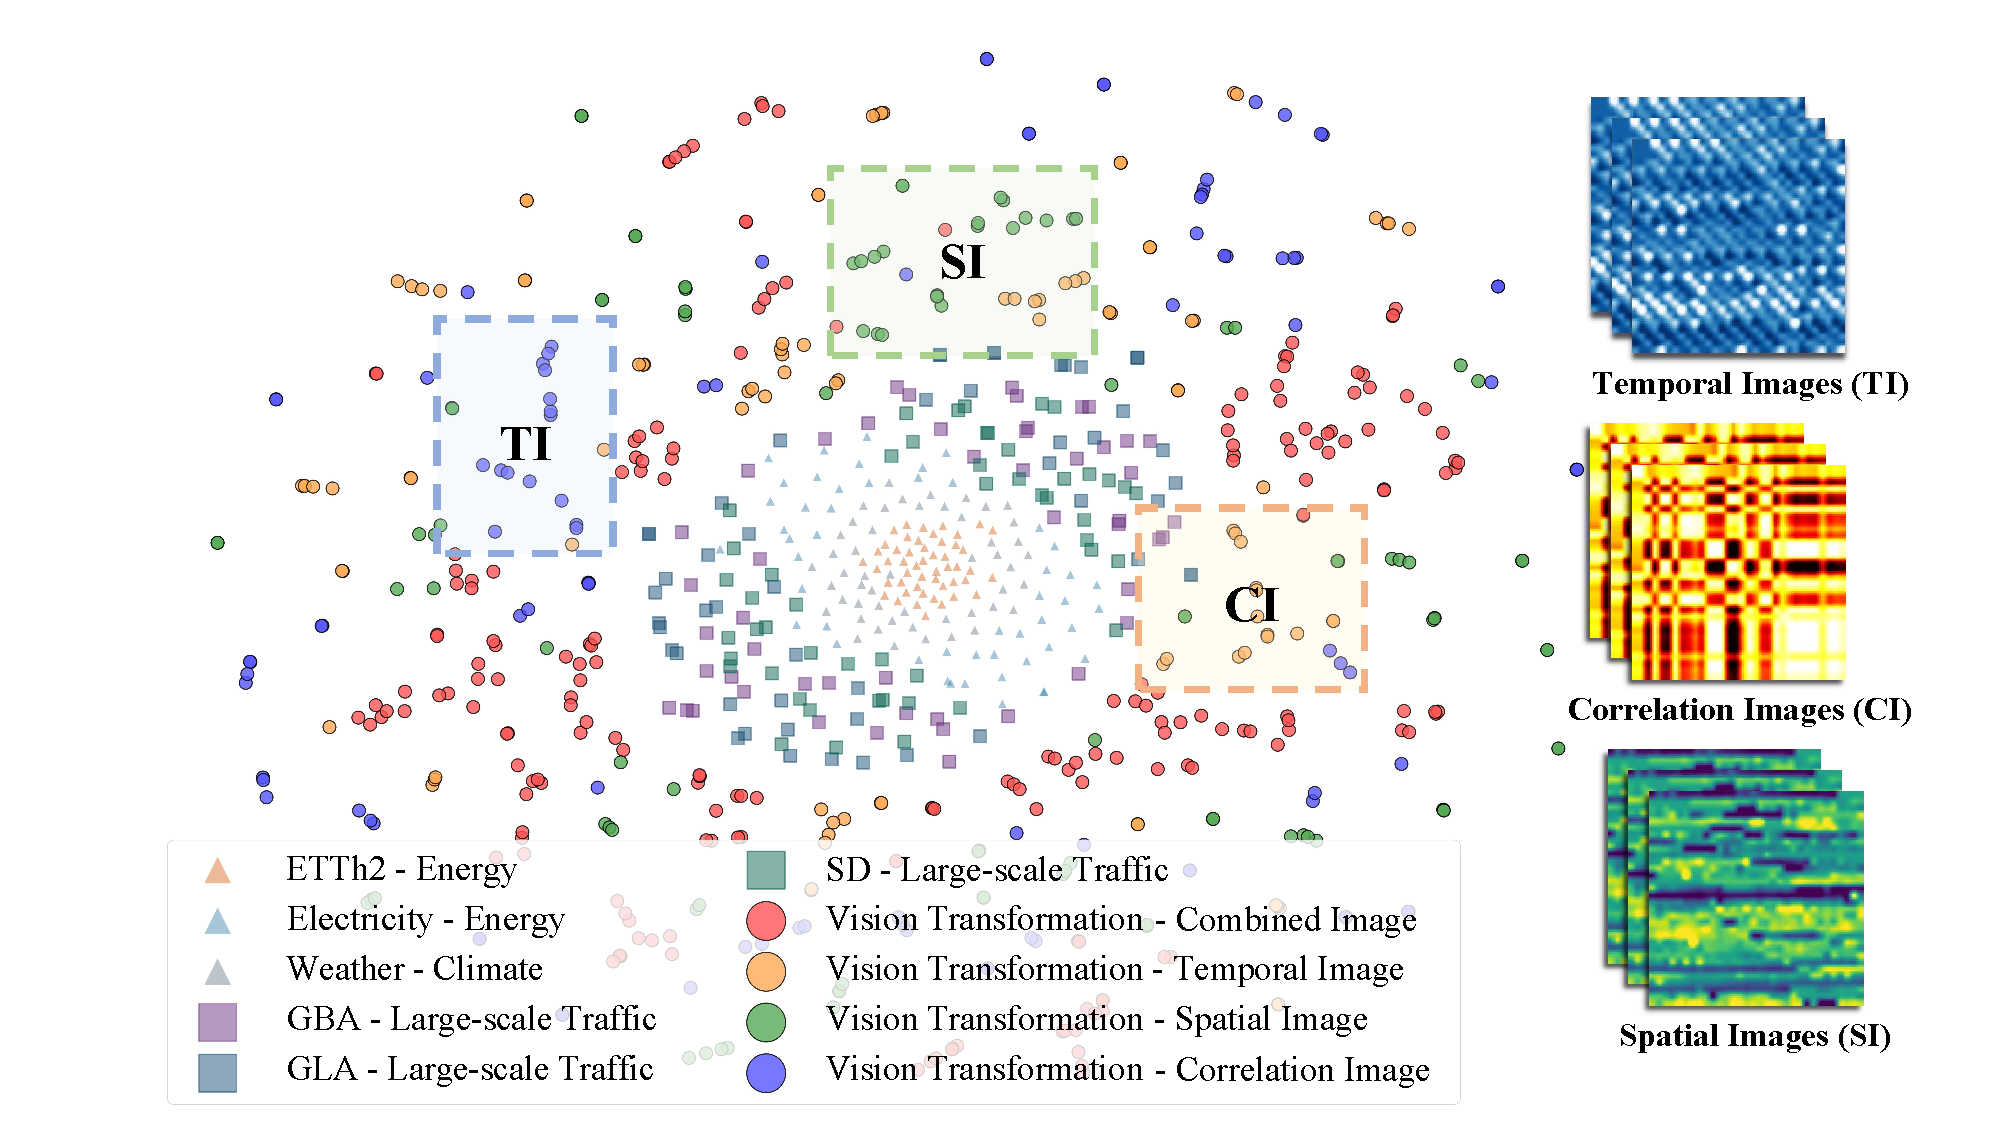
\includegraphics[width=0.48\textwidth]{figures/visualizations.pdf}
  %{figures/tsne_visualization.pdf}
  \caption{The t-SNE visualization of multi-domain data and our transformed visual embeddings. These visual representations cover large-scale traffic data and span other domains like climate and energy with constructed adjacent matrices, validating our approach's capability to reconstruct meaningful visual representations from ST data, and making complex spatio-temporal dependencies more interpretable through the visual modality.}
  \label{fig:tsne}
\end{figure}

\section{Limitation and Future Work}
While \model demonstrates superior performance across multiple domains, several limitations warrant acknowledgment and provide directions for future enhancement. Our current evaluation primarily focuses on established traffic flow, while the framework's generalizability to more complex domains such as epidemic dynamics, urban evolution patterns, or multi-scale environmental monitoring remains to be thoroughly validated. Additionally, the multi-view vision transformation process involves numerous hyperparameters for image processing, which require careful domain-specific tuning despite our comprehensive sensitivity analysis.

In future work, we will explore more effective approaches for transforming spatio-temporal data into visual modality, including learnable transformation functions and masked reconstruction strategies that could enable more adaptive and domain-specific visual representations while leveraging self-supervised learning paradigms. We will investigate the integration of our vision transformation approach with large-scale pre-trained Vision-Language Models (VLMs) such as CLIP, BLIP, and GPT-4V, potentially enabling zero-shot or few-shot adaptation to new spatio-temporal domains by harnessing the rich visual and textual understanding capabilities of these foundation models.

\section{Pseudo Code of ViST}
\label{appx:pseudo}
\begin{algorithm}[H]
\caption{Vision-enhanced Spatio-Temporal Forecasting}
\label{alg:vist}
\begin{algorithmic}[1]
    \REQUIRE Historical observations $\mathbf{X}\!\in\!\mathbb{R}^{B\times T\times N\times D}$,
             adjacency $\mathbf{A}\!\in\!\mathbb R^{N\times N}$,
             description text $\mathcal{D}$
    \ENSURE  Forecast $\widehat{\mathbf{Y}}\!\in\!\mathbb R^{B\times H'\times N\times \mathcal{D}'}$
    \Function{STIM}{\mathbf{X},\mathbf{A}}
        \STATE $\mathbf{E}_{\text{node}}\leftarrow\text{NodeEmbed}(\mathbf{X,A})$
        \STATE $(\mathbf{E}_{\text{tod}},\mathbf{E}_{\text{dow}})\leftarrow\text{TimeEmbed}(\mathbf{X})$
        \STATE $\mathbf{E}_{\text{adp}}\leftarrow\text{Conv}(\mathbf{X})$
        \STATE $\mathbf{H}_t\!\leftarrow\!\text{Conv}\bigl(
               \sigma(\mathbf{E}_{\text{adp}})
               \,\|\,\sigma(\mathbf{E}_{\text{node}})
               \,\|\,\sigma(\mathbf{E}_{\text{tod}})
               \,\|\,\sigma(\mathbf{E}_{\text{dow}})
               \bigr)$
        \RETURN $\mathbf{H_t}$
    %\EndFunction
    \Function{MVE}{\mathbf{H}_t,\mathbf{X},\mathbf{A}}
        % \STATE $\mathbf{V}_s\leftarrow\text{SCG}(\mathbf{X},\mathbf{A})$
        % \STATE $\mathbf{V}_t\leftarrow\text{TCG}(\mathbf{X})$
        % \STATE $\mathbf{V}_c\leftarrow\text{CCG}(\mathbf{X},\mathbf{H}_t,\mathbf{A})$
        %\STATE $\mathbf{V}_s, \mathbf{V}_t, \mathbf{V}_c \leftarrow\text{SCG}(\mathbf{X},\mathbf{A}),\text{TCG}(\mathbf{X}),\text{CCG}(\mathbf{X},\mathbf{H}_t,\mathbf{A})$
        % \STATE $\mathbf{V}\leftarrow[\mathbf{V}_s;\mathbf{V}_t;\mathbf{V}_c]$ % \Comment{concat on channel}
        \STATE $\mathbf{V}\leftarrow [\text{SCG}(\mathbf{X},\mathbf{A});\text{TCG}(\mathbf{X});\text{CCG}(\mathbf{X},\mathbf{H}_t,\mathbf{A})]$
        
        \RETURN $\mathbf{V}$
    %\EndFunction
    \Function{ConditionGeneration}{\mathbf{X},\mathbf{A},\mathcal{D}}
        \STATE $\mathbf{C}_g\leftarrow\text{MultiScaleGraph}(\mathbf{A},\mathbf{X})$
        \STATE $\mathbf{C}_t\leftarrow\text{TextEncoder}(\text{Prompt}(\mathbf{X},\mathcal{D}))$
        \RETURN $(\mathbf{C}_g,\mathbf{C}_t)$
    %\EndFunction
    \Function{CVFR}{\mathbf{V},\mathbf{C}_g,\mathbf{C}_t}
        \STATE $\mathbf{F}_{\text{temp}}\leftarrow\Phi_{\text{temp}}(\mathbf{V})$
        \STATE $\mathbf{F}_{\text{str}}\leftarrow\Phi_{\text{str}}\bigl([\mathbf{F}_{\text{temp}};\mathbf{C}_t]\bigr)$
        \STATE $\mathbf{F}_{\text{text}}\leftarrow\Phi_{\text{text}}\bigl([\mathbf{F}_{\text{str}};\sigma(\mathbf{C}_g)]\bigr)$
        \STATE $\mathbf{H}_v\leftarrow\text{Reshape}\!\bigl(\Phi_{\text{vis}}(\mathbf{V},\mathbf{F}_{\text{text}})\bigr)$
        \RETURN $\mathbf{H}_v$
    %%\EndFunction
    \Function{CrossModalFusion}{\mathbf{H}_t,\mathbf{H}_v}
        \STATE $\{\mathbf{H}_v^{(j)}\}, \{\mathbf{H}_t^{(i)}\} \leftarrow\text{BlockPartition}(\mathbf{H}_v,\mathbf{H}_t)$
        \FORALL{paired blocks $(i,j)$}
            \STATE $\widehat{\mathbf{H}}_t^{(i)}\leftarrow\text{Attention}(
\mathbf{H}_t^{(i)},\mathbf{H}_v^{(j)},\mathbf{H}_v^{(j)})$
            \STATE $\widehat{\mathbf{H}}_v^{(j)}\leftarrow\text{Attention}(                   \mathbf{H}_v^{(j)},\mathbf{H}_t^{(i)},\mathbf{H}_t^{(i)})$
        \ENDFOR
        \STATE $g_t,g_v\leftarrow\text{Softmax}\bigl(\text{MLP}([\widehat{\mathbf{H}}_t;\widehat{\mathbf{H}}_v])\bigr)$
        \STATE $\mathbf{H}_g\leftarrow g_t\!\cdot\!\widehat{\mathbf{H}}_t
                      + g_v\!\cdot\!\widehat{\mathbf{H}}_v$
        \STATE $\mathbf{H}_f\leftarrow\text{FFN}(\text{LayerNorm}(\mathbf{H}_g))+\mathbf{H}_g$
        \RETURN $\mathbf{H}_f$
    %\EndFunction
    \FORALL{mini-batch $(\mathbf{X},\mathbf{A},\mathcal{D},\mathbf{Y})$}
        \STATE $\mathbf{H}_t\leftarrow$\text{STIM}$(\mathbf{X},\mathbf{A})$
        \STATE $\mathbf{V}\leftarrow$\text{MVE}$(\mathbf{H}_t,\mathbf{X},\mathbf{A})$
        \STATE $(\mathbf{C}_g,\mathbf{C}_t)\leftarrow$\text{ConditionGen}$(\mathbf{X},\mathbf{A})$
        \STATE $\mathbf{H}_v\leftarrow$\text{CVFR}$(\mathbf{V},\mathbf{C}_g,\mathbf{C}_t)$
        \STATE $\mathbf{H}_f\leftarrow$\text{CrossModalFusion}$(\mathbf{H}_t,\mathbf{H}_v)$
        \STATE $\widehat{\mathbf{Y}}\leftarrow\text{MLP}(\text{Conv}(\mathbf{H}_f))$
        \STATE $\mathcal L\leftarrow\text{MaskedMAE}(\widehat{\mathbf{Y}},\mathbf{Y})$
        \STATE Update parameters with Adam using $\mathcal L$
    \ENDFOR
\end{algorithmic}
\end{algorithm}



\end{document}
